\documentclass{jarticle}
\usepackage[dvipdfmx]{graphicx}
\usepackage{here}
\usepackage{listings,jlisting} %日本語のコメントアウトをする場合jlistingが必要
%ここからソースコードの表示に関する設定
\lstset{
	basicstyle={\ttfamily},
		identifierstyle={\small},
		commentstyle={\smallitshape},
		keywordstyle={\small\bfseries},
		ndkeywordstyle={\small},
		stringstyle={\small\ttfamily},
		frame={tb},
		breaklines=true,
		columns=[l]{fullflexible},
		numbers=left,
		xrightmargin=0zw,
		xleftmargin=3zw,
		numberstyle={\scriptsize},
		stepnumber=1,
		numbersep=1zw,
		lineskip=-0.5ex
}
\title{個人開発進歩報告書}
\author{6119019056 山口力也}
\date{2019/07/02日提出}


\begin{document}
\maketitle
\section{進歩状況}
2019年6月25日\~7月2日までの進歩状況を説明する.

\subsection{進展事項}
まずはじめにスタート画面の作成を行った.後々作業がしやすくなるようにヘッダファイルを用いてメインプログラム、ウィンドウ表示などのプログラムを分割化し,関数などもわけた.
以下表\ref{table:bunkatu}に現状のプログラムの構成を示す.

\begin{table}[H]
\caption{プログラムの分割}
	\begin{center}
		\begin{tabular}{|c|c|c|}\hline \hline
		 ファイル名 &関数 & 機能 \\ \hline
		main.c & main & それぞれの関数を呼び出す \\ \hline 
		others.c & startup &メインウィンドウを作成 \\ 
		 & quits& 終了処理 \\ 
		& frames & フレームレートを調整 \\ 
		& background & 背景を作成\\ 
		& imageload & 画像を読み込み\\ 
		& drawtitle & タイトルを描画 \\ \hline
		\end{tabular}
	\end{center}
\label{table:bunkatu} 
\end{table}

\subsection{現状の課題}
現状の課題は山ほどあるが,優先度の高いものを以下に示す.

\section{今後の予定}
開発期間2019年7月2日\~7月9日の予定を以下に示す.

 
\begin{itemize}
\begin{item}
\item 背景の描画
\item タイトルの表示
\item キャラの描画
\end{item}
\end{itemize}
以下図\ref{fig:chart}にガントチャート図を示す.


\begin{figure}[H]
\begin{center}
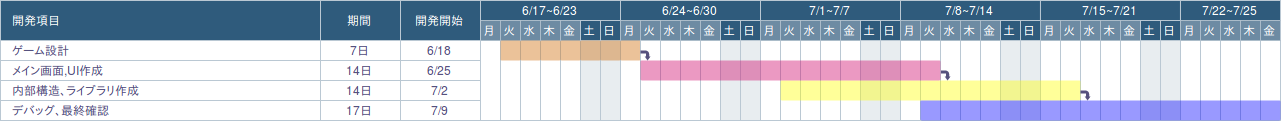
\includegraphics[width=7.0cm]{chart.png}
\caption{ガントチャート図}
\label{fig:chart}
\end{center}
\end{figure}


\end{document}

